\subsubsection{monolith::component::widget::BaseWidgetView}

\label{monolith::component::widget::BaseWidgetView}
\begin{figure}[ht]
	\centering
	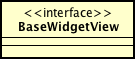
\includegraphics[scale=0.5]{Sezioni/SottosezioniST/img/BaseWidgetView.png}
	\caption{monolith::component::widget::BaseWidgetView}
\end{figure}

\begin{itemize}
\item \textbf{Descrizione:} Interfaccia che estende BaseComponent che rappresenta un qualsiasi widget che può essere inserito all'interno di un layout.
\item \textbf{Utilizzo:} Interfaccia che viene utilizzata ed implementata ogniqualvolta uno sviluppatore intende creare una nuova tipologia di widget che è possibile inserire all'interno di un layout.
\item \textbf{Attributi:}
\item \textbf{Metodi:}
\end{itemize}

\subsubsection{monolith::component::widget::button::ButtonWidgetView}

\label{monolith::component::widget::button::ButtonWidgetView}
\begin{figure}[ht]
	\centering
	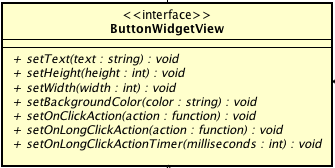
\includegraphics[scale=0.5]{Sezioni/SottosezioniST/img/ButtonWidgetView.png}
	\caption{monolith::component::widget::button::ButtonWidgetView}
\end{figure}

\begin{itemize}
\item \textbf{Descrizione}: Questa interfaccia rappresenta la view relativa ai widget di tipo bottone.
\item \textbf{Utilizzo}: L'interfaccia viene utilizzata per disaccoppiare presenter e implementazione del widget e per visualizzare i dati che gli vengono passati dal presenter.
\item \textbf{Attributi}:
\item \textbf{Metodi}:
	\begin{itemize}
	\item \textit{public setText(text:string):void}\\
	Imposta il testo all'interno del bottone.
		\\ \textbf{Parametri}: \begin{itemize}
		\item \textit{text:string}\\
		Rappresenta il testo che verrà impostato all'interno del bottone.
		\end{itemize}
	\item \textit{public setHeight(height:int):void}\\
	Imposta l'altezza del bottone.
		\\ \textbf{Parametri}: \begin{itemize}
		\item \textit{height:int}\\
		Rappresenta il numero di pixel corrispondente all'altezza del bottone che verrà impostata.
		\end{itemize}
	\item \textit{public setWidth(width:int):void}\\
	Imposta la larghezza del bottone.
		\\ \textbf{Parametri}: \begin{itemize}
		\item \textit{width:int}\\
		Rappresenta il numero di pixel corrispondente alla larghezza del bottone che verrà impostata.
		\end{itemize}
	\item \textit{public setBackgroundColor(color:string):void}\\
	Imposta il colore di sfondo del bottone.
		\\ \textbf{Parametri}: \begin{itemize}
		\item \textit{color:string}\\
		Rappresenta la stringa in esadecimale corrispondente al colore che verrà impostata come sfondo del bottone.
		\end{itemize}
	\item \textit{public setOnClickAction(action:function):void}\\
	Questo metodo viene utilizzato per impostare l'azione che deve essere eseguita dopo il click normale del bottone.
		\\ \textbf{Parametri}: \begin{itemize}
		\item \textit{action:function}\\
		L'azione, sotto forma di funzione, che deve essere eseguita al click normale del bottone.
		\end{itemize}
	\item \textit{public setOnLongClickAction(action:function):void}\\
		Questo metodo viene utilizzato per impostare l'azione che deve essere eseguita dopo il click prolungato del bottone.
		\\ \textbf{Parametri}: \begin{itemize}
		\item \textit{action:function}\\
		L'azione, sotto forma di funzione, che deve essere eseguita al click prolungato del bottone.
		\end{itemize}
		\item \textit{public setOnLongClickActionTimer(milliseconds:int):void}\\
		Questo metodo viene utilizzato per impostare il tempo che deve scorrere tra l'inizio della pressione del bottone affinché sia eseguita l'azione di click prolungato.
				\item{\textbf{Parametri}: \begin{itemize}
				\item \textit{milliseconds:int}\\
				Tempo in millisecondi che deve trascorrere dall'inizio della pressione sul bottone.
	\end{itemize}}
	\item \textit{public getHeight():string}\\
	Ritorna l'altezza del bottone.
	\item \textit{public getWidth():string}\\
	Ritorna la larghezza del bottone.
	\item \textit{public getColor():string}\\
	Ritorna la stringa che rappresenta il colore del bottone in esadecimale.
	\item \textit{public getText():string}\\
	Ritorna il testo contenuto all'interno del bottone.
	\end{itemize}
\item \textbf{Eventi}:
\end{itemize}

\subsubsection{monolith::component::widget::button::view::ButtonWidget}

\label{monolith::component::widget::button::view::ButtonWidget}
\begin{figure}[H]
	\centering
	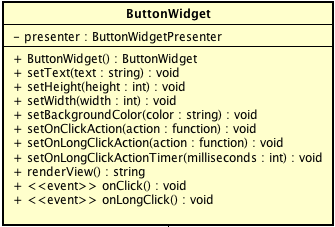
\includegraphics[scale=0.5]{Sezioni/SottosezioniST/img/ButtonWidget.png}
	\caption{monolith::component::widget::button::view::ButtonWidget}
\end{figure}

\begin{itemize}
\item \textbf{Descrizione}: Questa classe rappresenta un widget buttone, implementando l'interfaccia ButtonWidgetView.
\item \textbf{Utilizzo}: Implementando i metodi di ButtonWidgetView questa classe viene utilizzata al momento della creazione e della personalizzazione del bottone e delle sue reazioni alle azioni degli utenti.
\item \textbf{Attributi}: 
	\begin{itemize}
	\item \textit{private presenter:ButtonWidgetPresenter}\\
	Il presenter associato al widget bottone, al quale questa classe delega la gestione del comportamento del widget stesso.
	\item \textit{private eventClick:ClickButtonEvent}\\
	L'oggetto che si occupa della gestione degli eventi emessi dal ButtonWidget.
	\end{itemize}
\item \textbf{Metodi}:
	\begin{itemize}
	\item \textit{ButtonWidget():ButtonWidget}\\
	Il costruttore della classe ButtonWidget.
	\item \textit{public renderView():HtmlDOMElement}\\
	 Restituisce l'elemento DOM rappresentante il widget.
	\item \textit{public setText(text:string):void}\\
	Imposta il testo all'interno del bottone.
		\\ \textbf{Parametri}: \begin{itemize}
		\item \textit{text:string}\\
		Rappresenta il testo che verrà impostato all'interno del bottone.
		\end{itemize}
	\item \textit{public setHeight(height:int):void}\\
	Imposta l'altezza del bottone.
		\\ \textbf{Parametri}: \begin{itemize}
		\item \textit{height:int}\\
		Rappresenta il numero di pixel corrispondente all'altezza del bottone che verrà impostata.
		\end{itemize}
	\item \textit{public setWidth(width:int):void}\\
	Imposta la larghezza del bottone.
		\\ \textbf{Parametri}: \begin{itemize}
		\item \textit{width:int}\\
		Rappresenta il numero di pixel corrispondente alla larghezza del bottone che verrà impostata.
		\end{itemize}
	\item \textit{public setBackgroundColor(color:string):void}\\
	Imposta il colore di sfondo del bottone.
		\\ \textbf{Parametri}: \begin{itemize}
		\item \textit{color:string}\\
		Rappresenta la stringa in esadecimale corrispondente al colore che verrà impostata come sfondo del bottone.
		\end{itemize}
	\item \textit{public setOnClickAction(action:function):void}\\
	Questo metodo viene utilizzato per impostare l'azione che deve essere eseguita dopo il click normale del bottone.
		\\ \textbf{Parametri}: \begin{itemize}
		\item \textit{action:function}\\
		L'azione, sotto forma di funzione, che deve essere eseguita al click normale del bottone.
		\end{itemize}
	\item \textit{public setOnLongClickAction(action:function):void}\\
		Questo metodo viene utilizzato per impostare l'azione che deve essere eseguita dopo il click prolungato del bottone.
		\\ \textbf{Parametri}: \begin{itemize}
		\item \textit{action:function}\\
		L'azione, sotto forma di funzione, che deve essere eseguita al click prolungato del bottone.
		\end{itemize}
	\item \textit{public setOnLongClickActionTimer(milliseconds:int):void}\\
		Questo metodo viene utilizzato per impostare il timer per la pressione prolungata di un bottone.
				\\ \textbf{Parametri}: \begin{itemize}
				\item \textit{milliseconds:int}\\
				Tempo in millisecondi.
	\end{itemize}
	\item \textit{public getEvent():ClickButtonEvent}\\
	Ritorna l'oggetto che si occupa della gestione degli eventi emessi dal ButtonWidget.
	\item \textit{public getHeight():string}\\
	Ritorna l'altezza del bottone.
	\item \textit{public getWidth():string}\\
	Ritorna la larghezza del bottone.
	\item \textit{public getColor():string}\\
	Ritorna la stringa che rappresenta il colore del bottone in esadecimale.
	\item \textit{public getText():string}\\
	Ritorna il testo contenuto all'interno del bottone.
	\end{itemize}
\item{Eventi}:
\end{itemize}

\subsubsection{monolith::component::widget::button::presenter::ButtonWidgetPresenter}

\label{monolith::component::widget::button::presenter::ButtonWidgetPresenter}
\begin{figure}[H]
	\centering
	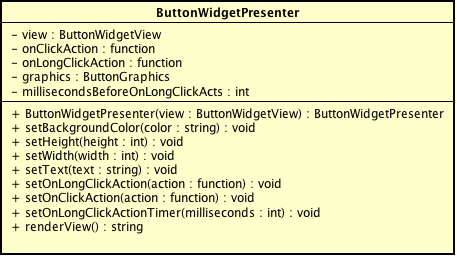
\includegraphics[scale=0.5]{Sezioni/SottosezioniST/img/ButtonWidgetPresenter.png}
	\caption{monolith::component::widget::button::presenter::ButtonWidgetPresenter}
\end{figure}

\begin{itemize}
\item \textbf{Descrizione}: Questa classe rappresenta il presenter per i widget di tipo bottone.
\item \textbf{Utilizzo}: Il presenter fa da tramite tra l'implementazione del widget e la view, formattando i dati che verranno visualizzati nella view e manipolando gli input dell'utente per eseguire le operazioni predisposte.
\item \textbf{Attributi}:
	\begin{itemize}
	\item \textit{private view:ButtonWidgetView}\\
	La view associata al presenter.
	\item \textit{private onClickAction:function}\\
	La funzione che il bottone eseguirà in seguito a un click normale.
	\item \textit{private onLongClicAction}\\
	La funzione che il bottone eseguirà in seguito a un click prolungato.
	\item \textit{private graphics:ButtonGraphics}\\
	L'oggetto che contiene le informazioni sullo stile visuale del bottone.
	\item \textit{private millisecondsBeforeOnLongClickActs:int}\\
	Tempo di pressione di un bottone in millisecondi dopo cui eseguire azioni in seguito ad un click prolungato.
	\item \textit{private dom:HtmlDOMElement}\\
	L'elemento dom che contiene il widget bottone in questione.
	\end{itemize}
\item \textbf{Metodi}:
	\begin{itemize}
	\item \textit{ButtonWidgetPresenter(view:ButtonWidgetView):ButtonWidgetPresenter}\\
	Il costruttore della classe ButtonWidgetPresenter.
		\\ \textbf{Parametri}: \begin{itemize}
		\item \textit{view:ButtonWidgetView}\\
		La view necessaria alla costruzione del presenter.
		\end{itemize}
	\item \textit{public setOnClickAction(action:function):void}\\
	Questo metodo viene utilizzato per impostare l'azione che deve essere eseguita dopo il click normale del bottone.
		\\ \textbf{Parametri}: \begin{itemize}
		\item \textit{action:function}\\
		L'azione, sotto forma di funzione, che deve essere eseguita al click normale del bottone.
		\end{itemize}
	\item \textit{public setOnLongClickAction(action:function):void}\\
		Questo metodo viene utilizzato per impostare l'azione che deve essere eseguita dopo il click prolungato del bottone.
		\\ \textbf{Parametri}: \begin{itemize}
		\item \textit{action:function}\\
		L'azione, sotto forma di funzione, che deve essere eseguita al click prolungato del bottone.
		\end{itemize}
		\item \textit{public setOnLongClickActionTimer(milliseconds:int):void}\\
		Questo metodo viene utilizzato per impostare il timer per la pressione prolungata di un bottone.
				\\ \textbf{Parametri}: \begin{itemize}
				\item \textit{milliseconds:int}\\
				Tempo in millisecondi.
	\end{itemize}
	\item \textit{public setText(string text:int):void}\\
	Imposta il testo all'interno del bottone
		\\ \textbf{Parametri}: \begin{itemize}
		\item \textit{text:string}\\
		Rappresenta il testo che verrà impostato all'interno del bottone.
		\end{itemize}
	\item \textit{public setHeight(height:int):void}\\
	Imposta l'altezza del bottone.
		\\ \textbf{Parametri}: \begin{itemize}
		\item \textit{height:int}\\
		Rappresenta il numero di pixel corrispondente all'altezza del bottone che verrà impostata.
		\end{itemize}
	\item \textit{public setWidth(width:int):void}\\
	Imposta la larghezza del bottone.
		\\ \textbf{Parametri}: \begin{itemize}
		\item \textit{width:int}\\
		Rappresenta il numero di pixel corrispondente alla larghezza del bottone che verrà impostata.
		\end{itemize}
	\item \textit{public setBackgroundColor(color:string):void}\\
	Imposta il colore di sfondo del bottone.
		\\ \textbf{Parametri}: \begin{itemize}
		\item \textit{color:string}\\
		Rappresenta la stringa in esadecimale corrispondente al colore che verrà impostata come sfondo del bottone.
		\end{itemize}\\
	\item \textit{public getHeight():string}\\
	Ritorna l'altezza del bottone.
	\item \textit{public getWidth():string}\\
	Ritorna la larghezza del bottone.
	\item \textit{public getColor():string}\\
	Ritorna la stringa che rappresenta il colore del bottone in esadecimale.
	\item \textit{public getText():string}\\
	Ritorna il testo contenuto all'interno del bottone.
	\item \textit{public renderView():HtmlDOMElement}\\
	Restituisce l'elemento DOM rappresentante il widget.
	\end{itemize}
\end{itemize}

\subsubsection{monolith::component::widget::button::option::ButtonGraphics}

\label{monolith::component::widget::button::option::ButtonGraphics}
\begin{figure}[H]
	\centering
	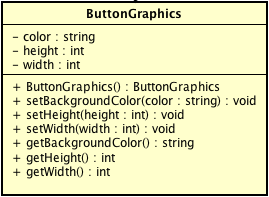
\includegraphics[scale=0.5]{Sezioni/SottosezioniST/img/ButtonGraphics.png}
	\caption{monolith::component::widget::button::option::ButtonGraphics}
\end{figure}

\begin{itemize}
\item \textbf{Descrizione}: Questa classe rappresenta l'aspetto visivo del bottone.
\item \textbf{Utilizzo}:
\item \textbf{Attributi}:
	\begin{itemize}
	\item \textit{private color:string}\\
	Rappresenta la stringa in esadecimale corrispondente al colore che verrà impostata come sfondo del bottone.
	\item \textit{private height:int}\\
	Rappresenta il numero di pixel corrispondente all'altezza del bottone. 
	\item \textit{private width:int}\\
	Rappresenta il numero di pixel corrispondente alla larghezza del bottone.
	\end{itemize}
\item \textbf{Metodi}:
	\begin{itemize}
	\item \textit{ButtonGraphics():ButtonGraphics}\\
	Il costruttore della classe ButtonGraphics.
	\item \textit{public setHeight(height:int):void}\\
	Imposta l'altezza del bottone.
		\\ \textbf{Parametri}: \begin{itemize}
		\item \textit{height:int}\\
		Rappresenta il numero di pixel corrispondente all'altezza del bottone che verrà impostata.
		\end{itemize}
	\item \textit{public setWidth(width:int):void}\\
	imposta la larghezza del bottone.
		\\ \textbf{Parametri}: \begin{itemize}
		\item \textit{width:int}\\
		Rappresenta il numero di pixel corrispondente alla larghezza del bottone che verrà impostata.
		\end{itemize}
	\item \textit{public setBackgroundColor(color:string):void}\\
	imposta il colore di sfondo del bottone.
		\\ \textbf{Parametri}: \begin{itemize}
		\item \textit{color:string}\\
		Rappresenta la stringa in esadecimale corrispondente al colore che verrà come sfondo del bottone.
		\end{itemize}
	\item \textit{public getHeight():int}\\
	Ritorna l'altezza del bottone.
	\item \textit{public getWidth():int}\\
	Ritorna la larghezza del bottone.
	\item \textit{public getBackgroundColor():string}\\
	Ritorna la stringa in esadecimale corrispondente al colore di sfondo del bottone.
	\end{itemize}
\end{itemize}

\subsubsection{monolith::component::widget::text::TextWidgetView}

\label{monolith::component::widget::text::TextWidgetView}
\begin{figure}[H]
	\centering
	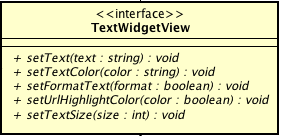
\includegraphics[scale=0.5]{Sezioni/SottosezioniST/img/TextWidgetView.png}
	\caption{monolith::component::widget::text::TextWidgetView}
\end{figure}

\begin{itemize}
\item \textbf{Descrizione}: Questa interfaccia rappresenta la view relativa ai widget di tipo testo.
\item \textbf{Utilizzo}: L'interfaccia viene utilizzata per disaccoppiare presenter e implementazione del widget e per visualizzare i dati che gli vengono passati dal presenter.
\item \textbf{Attributi}:
\item \textbf{Metodi}:
	\begin{itemize}
	\item \textit{public setText(text:string):void}\\
	Imposta il testo all'interno del widget testo.
		\\ \textbf{Parametri}: \begin{itemize}
		\item \textit{text:string}\\
		Rappresenta con una string il testo che va inserito all'interno del widget.
		\end{itemize}
	\item \textit{public setTextColor(color:string):void}\\
	Imposta il colore del testo del widget testo.
		\\ \textbf{Parametri}: \begin{itemize}
		\item \textit{color:string}\\
		Rappresenta la stringa in esadecimale corrispondente al colore che verrà come sfondo del bottone.
		\end{itemize}
	\item \textit{public setFormatText(format: boolean):void}\\
	Imposta il widget a testo formattato o testo semplice.
		\\ \textbf{Parametri}: \begin{itemize}
		\item \textit{format: boolean}\\
		Questo booleano viene impostato a true se si vuole il testo del widget formattato, a false altrimenti.
		\end{itemize} 
	\item \textit{public setUrlHighlightColor(color:boolean):void}\\
	Imposta la possibilità di cliccare o meno i link presenti nel testo del widget.
		\\ \textbf{Parametri}: \begin{itemize}
		\item \textit{color:string}\\
		Questo booleano viene impostato a true se si vogliono i link cliccabili, a false altrimenti.
		\end{itemize} 
	\item \textit{public setTextSize(size:int):void}\\
	Imposta la grandezza del testo nel widget
		\\ \textbf{Parametri}: \begin{itemize}
		\item \textit{size:int}\\
		Rappresenta il numero di pixel corrispondente all'altezza del testo che verrà impostata all'interno del widget.
		\end{itemize} 
	\item \textit{getColor():string}\\
	Ritorna il colore del testo all'interno del TextWidget.
	\item \textit{getText():string}\\
	Ritorna il testo contenuto all'interno del TextWidget.
	\end{itemize}
\end{itemize}

\subsubsection{monolith::component::widget::text::view::TextWidget}

\label{monolith::component::widget::text::view::TextWidget}
\begin{figure}[H]
	\centering
	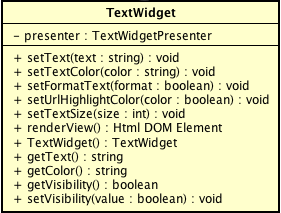
\includegraphics[scale=0.5]{Sezioni/SottosezioniST/img/TextWidget.png}
	\caption{monolith::component::widget::text::view::TextWidget}
\end{figure}

\begin{itemize}
\item \textbf{Descrizione}: Questa classe rappresenta un widget di testo, implementando l'interfaccia TextWidgetView
\item \textbf{Utilizzo}: Implementando i metodi di TextWidgetView questa classe viene utilizzata al momento della creazione e della personalizzazione del widget di testo e del suo contenuto.
\item \textbf{Attributi}:
	\begin{itemize}
	\item \textit{private presenter:TextWidgetPresenter}\\
	Il presenter associato al widget testo, al quale questa classe delega la gestione del comportamento del widget stesso.
	\end{itemize}
\item \textbf{Metodi}:
	\begin{itemize}
	\item \textit{public TextWidget():TextWidget}\\
	Il costruttore della classe TextWidget.
	\item \textit{public setText(text:string):void}\\
	Imposta il testo all'interno del widget testo.
		\\ \textbf{Parametri}: \begin{itemize}
		\item \textit{text:string}\\
		Rappresenta con una string il testo che va inserito all'interno del widget.
		\end{itemize} 
	\item \textit{public setTextColor(color:string):void}\\
	Imposta il colore del testo del widget testo.
		\\ \textbf{Parametri}: \begin{itemize}
		\item \textit{color:string}\\
		Rappresenta la stringa in esadecimale corrispondente al colore che verrà come sfondo del bottone.
		\end{itemize} 
	\item \textit{public setFormatText(format: boolean):void}\\
	Imposta il widget a testo formattato o testo semplice.
		\\ \textbf{Parametri}: \begin{itemize}
		\item \textit{format: boolean}\\
		Questo booleano viene impostato a true se si vuole il testo del widget formattato, a false altrimenti.
		\end{itemize} 
	\item \textit{public setUrlHighlightColor(color:boolean):void}\\
	Imposta la possiblità di cliccare o meno i link presenti nel testo del widget.
		\\ \textbf{Parametri}: \begin{itemize}
		\item \textit{color:string}\\
		Questo booleano viene impostato a true se si vogliono i link cliccabili, a false altrimenti.
		\end{itemize} 
	\item \textit{public setTextSize(size:int):void}\\
	Imposta la grandezza del testo nel widget
		\\ \textbf{Parametri}: \begin{itemize}
		\item \textit{size:int}\\
		Rappresenta il numero di pixel corrispondente all'altezza del testo che verrà impostata all'interno del widget.
		\end{itemize} 
	\item \textit{getColor():string}\\
	Ritorna il colore del testo all'interno del TextWidget.
	\item \textit{getText():string}\\
	Ritorna il testo contenuto all'interno del TextWidget.
	\item \textit{public renderView():HtmlDOMElement}\\
	Restituisce l'elemento DOM rappresentante il widget.
	\end{itemize}
\end{itemize}

\subsubsection{monolith::component::widget::text::presenter::TextWidgetPresenter}

\label{monolith::component::widget::text::presenter::TextWidgetPresenter}
\begin{figure}[H]
	\centering
	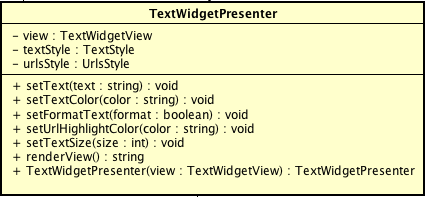
\includegraphics[scale=0.5]{Sezioni/SottosezioniST/img/TextWidgetPresenter.png}
	\caption{monolith::component::widget::text::presenter::TextWidgetPresenter}
\end{figure}

\begin{itemize}
\item \textbf{Descrizione}: Questa classe rappresenta il presenter per i widget di tipo testo.
\item \textbf{Utilizzo}: Il presenter fa da tramite tra l'implementazione del widget e la view,  formattando i dati che verranno visualizzati nella view.
\item \textbf{Attributi}:
	\begin{itemize}
	\item \textit{private view:TextWidgetView}\\
	La view associata al presenter.
	\item \textit{private textStyle:TextStyle}\\
	Stile del testo del widget.
	\item \textit{private urlsStyle:UrlsStyle}\\
	Stile dei link presenti all'interno del testo.
	\item \textit{private dom:HtmlDOMElement}\\
	L'elemento dom che contiene il widget testo in questione.
	\end{itemize}
\item \textbf{Metodi}:
	\begin{itemize}
	\item \textit{public TextWidgetPresenter(view:TextWidgetView):TextWidgetPresenter}\\
	Il costruttore della classe TextWidgetPresenter.
		\\ \textbf{Parametri}: \begin{itemize}
		\item \textit{view:TextWidgetView}\\
		La view necessaria alla costruzione del presenter.
		\end{itemize} 
	\item \textit{private updateText():void}\\
	Aggiorna il dom del widget in modo tale da mostrare le modifiche effettuate al testo contenuto al suo interno.
	\item \textit{private updateLinkColor():void}\\
	Aggiorna il dom del widget in modo tale da mostrare le modifiche effettuate al colore dei link contenuti all'interno del testo del widget.
	\item \textit{public setText(text:string):void}\\
	Imposta il testo all'interno del widget testo.
		\\ \textbf{Parametri}: \begin{itemize}
		\item \textit{text:string}\\
		Rappresenta con una string il testo che va inserito all'interno del widget.
		\end{itemize} 
	\item \textit{public setTextColor(color:string):void}\\
	Imposta il colore del testo del widget testo.
		\\ \textbf{Parametri}: \begin{itemize}
		\item \textit{color:string}\\
		Rappresenta la stringa in esadecimale corrispondente al colore che verrà impostato al testo all'interno del widget.
		\end{itemize} 
	\item \textit{public setFormatText(format: boolean):void}\\
	Imposta il widget a testo formattato o testo semplice.
		\\ \textbf{Parametri}: \begin{itemize}
		\item \textit{format: boolean}\\
		Questo booleano viene impostato a true se si vuole il testo del widget formattato, a false altrimenti.
		\end{itemize} 
	\item \textit{public setUrlHighlightColor(color:boolean):void}\\
	Imposta la possiblità di cliccare o meno i link presenti nel testo del widget.
		\\ \textbf{Parametri}: \begin{itemize}
		\item \textit{color:string}\\
		Questo booleano viene impostato a true se si vogliono i link cliccabili, a false altrimenti.
		\end{itemize} 
	\item \textit{public setTextSize(size:int):void}\\
	Imposta la grandezza del testo nel widget.
		\\ \textbf{Parametri}: \begin{itemize}
		\item \textit{size:int}\\
		Rappresenta il numero di pixel corrispondente all'altezza del testo che verrà impostata all'interno del widget.
		\end{itemize} 
	\item \textit{getColor():string}\\
	Ritorna il colore del testo all'interno del TextWidget.
	\item \textit{getText():string}\\
	Ritorna il testo contenuto all'interno del TextWidget.
	\item \textit{public renderView():HtmlDOMElement}\\
	Restituisce l'elemento DOM rappresentante il widget.
	\end{itemize}
\end{itemize}

\subsubsection{monolith::component::widget::text::option::TextStyle}

\label{monolith::component::widget::text::option::TextStyle}
\begin{figure}[H]
	\centering
	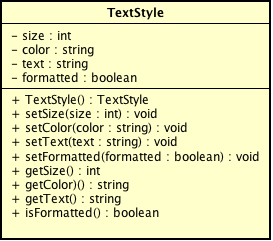
\includegraphics[scale=0.5]{Sezioni/SottosezioniST/img/TextStyle.png}
	\caption{monolith::component::widget::text::option::TextStyle}
\end{figure}

\begin{itemize}
\item \textbf{Descrizione}: Questa classe rappresenta lo stile del testo all'interno di un widget testo.
\item \textbf{Utilizzo}: La classe viene utilizzata ogniqualvolta vengono utilizzati metodi che cambiano lo stile visuale del testo in un widget testo.
\item \textbf{Attributi}:
	\begin{itemize}
	\item \textit{private size:int}\\
	Rappresenta il numero di pixel corrispondente all'altezza del testo.
	\item \textit{private color:string}\\
	Rappresenta la stringa in esadecimale corrispondente al colore del testo.
	\item \textit{private text:string}\\
	Rappresenta il testo stesso. 
	\item \textit{private formatted:boolean}\\
	Rappresenta l'impostazione del testo a formattato o meno.
	\end{itemize}
\item \textbf{Metodi}:
	\begin{itemize}
	\item \textit{public TextStyle():TextStyle}\\
	Il costruttore della classe TextStyle.
	\item \textit{public setSize(size:int):void}\\
	Imposta la grandezza del testo.
		\\ \textbf{Parametri}: \begin{itemize}
		\item \textit{size:int}\\
		Rappresenta il numero di pixel corrispondente all'altezza del testo che verrà impostata all'interno del widget.
		\end{itemize} 
	\item \textit{public setColor(color:string):void}\\
	Imposta il colore del testo del widget testo.
		\\ \textbf{Parametri}: \begin{itemize}
		\item \textit{color:string}\\
		Rappresenta la stringa in esadecimale corrispondente al colore che verrà impostato al testo all'interno del widget.
		\end{itemize} 
	\item \textit{public setText(string text:int):void}\\
	Imposta il testo.
		\\ \textbf{Parametri}: \begin{itemize}
		\item \textit{string text:int}\\
		Rappresenta con una string il testo che va inserito.
		\end{itemize} 
	\item \textit{public setFormatted(formatted:boolean):void}\\
	Imposta il testo a formattato o meno.
		\\ \textbf{Parametri}: \begin{itemize}
		\item \textit{formatted:boolean}\\
		Se questo booleano è a true il testo del widget viene formattato, se a false il testo viene considerato normale.
		\end{itemize} 
	\item \textit{public getSize():int}\\
	Ritorna il numero di pixel corrispondente all'altezza del testo.
	\item \textit{public getColor():string}\\
	Ritorna  la stringa in esadecimale corrispondente al colore del testo.
	\item \textit{public getText():string}\\
	Ritorna la stringa contenente il testo.
	\item \textit{public isFormatted():boolean}\\
	Ritorna true se il testo è formattato, false altrimenti.
	\end{itemize}
\end{itemize}

\subsubsection{monolith::component::widget::text::option::UrlStyle}

\label{monolith::component::widget::text::option::UrlsStyle}
\begin{figure}[H]
	\centering
	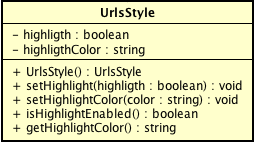
\includegraphics[scale=0.5]{Sezioni/SottosezioniST/img/UrlsStyle.png}
	\caption{monolith::component::widget::text::option::UrlsStyle}
\end{figure}

\begin{itemize}
\item \textbf{Descrizione}: Questa classe rappresenta lo stile del testo dei link all'interno di un widget testo.
\item \textbf{Utilizzo}: La classe viene utilizzata ogniqualvolta vengono utilizzati metodi che cambiano lo stile visuale dei link nel contenuto di un widget testo.
\item \textbf{Attributi}:
	\begin{itemize}
	\item \textit{private highlight:boolean}\\
	Booleano che rappresenta la possibilità o meno di cliccare i link nel testo.
	\item \textit{private highlightColor:string}\\
	Stringa in esadecimale corrispondente al colore dei link al testo all'interno del testo.
	\end{itemize}
\item \textbf{Metodi}:
	\begin{itemize}
	\item \textit{public UrlStyle():UrlsStyle}\\
	Il costruttore della classe UrlStyle.
	\item \textit{public setHighlight(color:boolean):void}\\
	Imposta la possiblità di cliccare o meno i link presenti nel testo.
		\\ \textbf{Parametri}: \begin{itemize}
		\item \textit{color:string}\\
		Questo booleano viene impostato a true se si vogliono i link cliccabili, a false altrimenti.
		\end{itemize} 
	\item \textit{public setHighlightColor(color:string):void}\\
	Imposta il colore del testo dei link presenti all'interno del testo.
		\\ \textbf{Parametri}: \begin{itemize}
		\item \textit{color:string}\\
		Rappresenta la stringa in esadecimale corrispondente al colore che verrà impostato per i link al testo all'interno del testo.
		\end{itemize} 
	\item \textit{public isHighlightEnabled():boolean}\\
	Ritorna true se i link sono cliccabili, false altrimenti.
	\item \textit{public getHighlightColor():string}\\
	Ritorna la stringa in esadecimale corrispondente al colore che verrà impostato per i link al testo all'interno del widget.
	\end{itemize}
\end{itemize}

\subsubsection{monolith::component::widget::checklist::ChecklistItemWidgetView}

\label{monolith::component::widget::checklist::ChecklistItemWidgetView}
\begin{figure}[H]
	\centering
	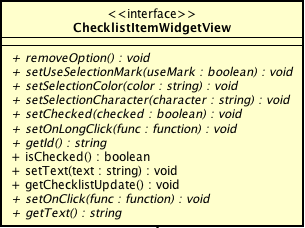
\includegraphics[scale=0.5]{Sezioni/SottosezioniST/img/ChecklistItemWidgetView.png}
	\caption{monolith::component::widget::checklist::ChecklistItemWidgetView}
\end{figure}

\begin{itemize}
\item \textbf{Descrizione}: Questa interfaccia rappresenta la view relativa ai widget di tipo checklistitem.
\item \textbf{Utilizzo}: L'interfaccia viene utilizzata per disaccoppiare presenter e implementazione del widget, visualizza i dati che gli vengono passati dal presenter.
\item \textbf{Attributi}:
\item \textbf{Metodi}:
	\begin{itemize}
	\item \textit{public removeOption():void}\\
	Questo metodo rimuove il ChecklistItemWidget dalla bolla in cui è stato inserito.
	\item \textit{public getId():string}\\
	Questo metodo ritorna l'identificativo del ChecklistItemWidget.
	\item \textit{public isChecked():boolean}\\
	Ritorna true se la entry è spuntata, false altrimenti.
	\item \textit{public setUseSelectionMark(useMark:boolean):void}\\
	Imposta la visualizzazione delle spunte con un carattere oppure con un colore.
		\\ \textbf{Parametri}: \begin{itemize}
		\item \textit{useMark:boolean}\\
		Se questo è a true la visualizzazione della spunta viene effettuata con un carattere, altrimenti la visualizzazione viene effettuata con un colore.
		\end{itemize}  
	\item \textit{public setSelectionColor(color:string):void}\\
	Imposta il colore con il quale effettuare la visualizzazione delle spunte.
		\\ \textbf{Parametri}: \begin{itemize}
		\item \textit{color:string}\\
		Rappresenta la stringa in esadecimale corrispondente al colore che verrà impostato per visualizzare le spunte.
		\end{itemize}  
	\item \textit{public setSelectionCharacter(character:string):void}\\
	Imposta il carattere utilizzato per la visualizzazione delle spunte.
		\\ \textbf{Parametri}: \begin{itemize}
		\item \textit{character:string}\\
		Il carattere utilizzato per la visualizzazione delle spunte.
		\end{itemize} 
	\item \textit{public setChecked(checked:boolean):void}\\
	Permette di spuntare un oggetto della checlist o di togliere una spunta da esso.
		\\ \textbf{Parametri}: \begin{itemize}
		\item \textit{checked:boolean}\\
		Questo booleano è a true se si vorrà spuntare la entry, a false altrimenti.
		\end{itemize}  
	\item \textit{public getChecklistUpdate():checklistUpdate}\\
	Questo metodo restituisce un oggetto di tipo checklistUpdate associato al ChecklistItemWidget in questione, che sarà utilizzato dal presenter per lanciare gli eventi di aggiornamento del widget.
	\item \textit{public setOnClick(func:function):void}\\
	Questo metodo viene utilizzato per impostare l'azione che deve essere eseguita dopo il click normale del widget.
		\\ \textbf{Parametri}: \begin{itemize}
		\item \textit{func:function}\\
		L'azione, sotto forma di funzione, che deve essere eseguita al click normale del bottone.
		\end{itemize}
	\item \textit{public setOnLongClick(func:function):void}\\
		Questo metodo viene utilizzato per impostare l'azione che deve essere eseguita dopo il click prolungato del widget.
		\\ \textbf{Parametri}: \begin{itemize}
		\item \textit{func:function}\\
		L'azione, sotto forma di funzione, che deve essere eseguita al click prolungato del bottone.
		\end{itemize}
	\item \texit{public setText(text:string):void}\\
	Imposta il testo presente all'interno del widget.
		\\ \textbf{Parametri}: \begin{itemize}
		\item \textit{text:string}\\
		Il testo da impostare nel checklistItem widget.
		\end{itemize}
	\item \texit{public getText():string}\\
	Ritorna il testo presente all'interno del ChecklistItemWidget
	\end{itemize}
\item{Eventi}:
\end{itemize}

\subsubsection{monolith::component::widget::checklist::view::ChecklistItemWidget}

\label{monolith::component::widget::checklist::view::ChecklistItemWidget}
\begin{figure}[H]
	\centering
	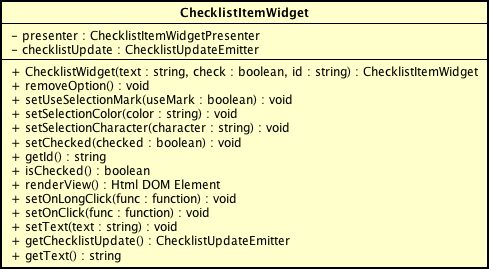
\includegraphics[scale=0.5]{Sezioni/SottosezioniST/img/ChecklistItemWidget.png}
	\caption{monolith::component::widget::checklist::view::ChecklistItemWidget}
\end{figure}

\begin{itemize}
\item \textbf{Descrizione}: Questa classe rappresenta un widget checklistItem, implementando l'interfaccia ChecklistItemWidgetView
\item \textbf{Utilizzo}: Implementando i metodi di ChecklistItemWidgetView questa classe viene utilizzata al momento della creazione e della personalizzazione del widget checklistItem e del suo contenuto.
\item \textbf{Attributi}:
	\begin{itemize}
	\item \textit{private presenter:ChecklistItemWidgetPresenter}\\
	Il presenter associato al widget checklistItem, al quale questa classe delega la gestione del comportamento del widget stesso.
	\item \textit{private checklistUpdate:ChecklistUpdateEmitter}\\
	Questo oggetto permette di catturare gli eventi di tipo update.
	\end{itemize}
\item \textbf{Metodi}:
	\begin{itemize}
	\item \textit{public removeOption():void}\\
	Questo metodo rimuove il ChecklistItemWidget dalla bolla in cui è stato inserito.
	\item \textit{public getId():string}\\
	Questo metodo ritorna l'identificativo del ChecklistItemWidget.
	\item \textit{public isChecked():boolean}\\
	Ritorna true se la entry è spuntata, false altrimenti.
	\item \textit{public setUseSelectionMark(useMark:boolean):void}\\
	Imposta la visualizzazione delle spunte con un carattere oppure con un colore.
		\\ \textbf{Parametri}: \begin{itemize}
		\item \textit{useMark:boolean}\\
		Se questo è a true la visualizzazione della spunta viene effettuata con un carattere, altrimenti la visualizzazione viene effettuata con un colore.
		\end{itemize}  
	\item \textit{public setSelectionColor(color:string):void}\\
	Imposta il colore con il quale effettuare la visualizzazione delle spunte.
		\\ \textbf{Parametri}: \begin{itemize}
		\item \textit{color:string}\\
		Rappresenta la stringa in esadecimale corrispondente al colore che verrà impostato per visualizzare le spunte.
		\end{itemize}  
	\item \textit{public setSelectionCharacter(character:string):void}\\
	Imposta il carattere utilizzato per la visualizzazione delle spunte.
		\\ \textbf{Parametri}: \begin{itemize}
		\item \textit{character:string}\\
		Il carattere utilizzato per la visualizzazione delle spunte.
		\end{itemize} 
	\item \textit{public setChecked(checked:boolean):void}\\
	Permette di spuntare un oggetto della checlist o di togliere una spunta da esso.
		\\ \textbf{Parametri}: \begin{itemize}
		\item \textit{checked:boolean}\\
		Questo booleano è a true se si vorrà spuntare la entry, a false altrimenti.
		\end{itemize}  
	\item \textit{public getChecklistUpdate():checklistUpdate}\\
	Questo metodo restituisce un oggetto di tipo checklistUpdate associato al ChecklistItemWidget in questione, che sarà utilizzato dal presenter per lanciare gli eventi di aggiornamento del widget.
	\item \textit{public setOnClick(func:function):void}\\
	Questo metodo viene utilizzato per impostare l'azione che deve essere eseguita dopo il click normale del widget.
		\\ \textbf{Parametri}: \begin{itemize}
		\item \textit{func:function}\\
		L'azione, sotto forma di funzione, che deve essere eseguita al click normale del bottone.
		\end{itemize}
	\item \textit{public setOnLongClick(func:function):void}\\
		Questo metodo viene utilizzato per impostare l'azione che deve essere eseguita dopo il click prolungato del widget.
		\\ \textbf{Parametri}: \begin{itemize}
		\item \textit{func:function}\\
		L'azione, sotto forma di funzione, che deve essere eseguita al click prolungato del bottone.
		\end{itemize}
	\item \texit{public setText(text:string):void}\\
	Imposta il testo presente all'interno del widget.
		\\ \textbf{Parametri}: \begin{itemize}
		\item \textit{text:string}\\
		Il testo da impostare nel checklistItem widget.
		\end{itemize}
	\item \texit{public getText():string}\\
	Ritorna il testo presente all'interno del ChecklistItemWidget
	\item \textit{public renderView():HtmlDOMElement}\\
	Restituisce l'elemento DOM rappresentante il widget.
	\end{itemize}
\item{Eventi}:
\end{itemize}

\subsubsection{monolith::component::widget::checklist::presenter::ChecklistItemWidgetPresenter}

\label{monolith::component::widget::checklist::presenter::ChecklistItemWidgetPresenter}
\begin{figure}[H]
	\centering
	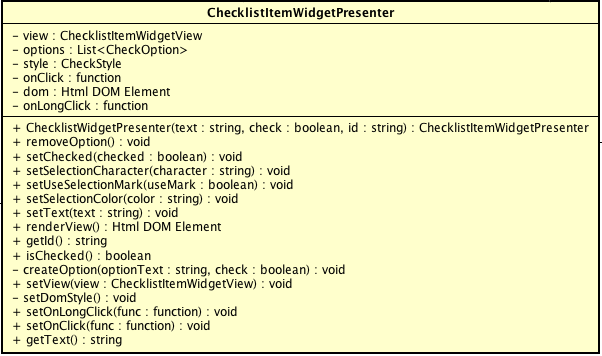
\includegraphics[scale=0.5]{Sezioni/SottosezioniST/img/ChecklistItemWidgetPresenter.png}
	\caption{monolith::component::widget::checklist::presenter::ChecklistItemWidgetPresenter}
\end{figure}

\begin{itemize}
\item \textbf{Descrizione}: Questa classe rappresenta il presenter per i widget di tipo checklistItem.
\item \textbf{Utilizzo}: Il presenter fa da tramite tra l'implementazione del widget e la view, formattando i dati che verranno visualizzati nella view e manipolando gli input dell'utente per eseguire le operazioni predisposte.
\item \textbf{Attributi}:
	\begin{itemize}
	\item \textit{private view:ChecklistWidgetView}\\
	La view associata al presenter.
	\item \textit{private dom:HtmlDOMElement}\\
	L'elemento dom che contiene il widget checklistItem in questione.
	\item \textit{private style:CheckStyle}\\
	Stile per le spunte della lista.
	\item \textit{private options:CheckOption}\\
	Rappresenta lo stato del widget.
	\item \textit{onClick:function}\\
	La funzione che deve essere eseguita dopo il click normale sul widget.
	\item \textit{onLongClick:function}\\
	La funzione che deve essere eseguita dopo il click prolungato (che ha timer predefinito a 1 secondo) sul widget.
	\end{itemize}
\item \textbf{Metodi}:
	\begin{itemize}
	\item \textit{public ChecklistItemWidgetPresenter(text:string,check:boolean,id:string):ChecklistItemWidgetPresenter}\\
		\\ \textbf{Parametri}: \begin{itemize}
		\item \textit{text:string}\\
		Il testo del widget.
		\item \textit{check:boolean}\\
		Il booleano che rapresenta lo stato della spunta del widget.
		\item \textit{id:string}\\
		L'identificativo del widget.
		\end{itemize}
	\item \textit{private createOption(optionText:string,check:boolean):void}\\
	Questo metodo crea il DOM del checklistItemWidget.
	\item \textit{private setDomStyle():void}\\
	Permette di aggiornare il DOM del widget.
	\item \textit{public setView(view:ChecklistItemWidgetView):void}\\
	Permette di impostare il riferimento alla view del presenter.
	\item \textit{public removeOption():void}\\
	Questo metodo rimuove il ChecklistItemWidget dalla bolla in cui è stato inserito.
	\item \textit{public getId():string}\\
	Questo metodo ritorna l'identificativo del ChecklistItemWidget.
	\item \textit{public isChecked():boolean}\\
	Ritorna true se la entry è spuntata, false altrimenti.
	\item \textit{public setUseSelectionMark(useMark:boolean):void}\\
	Imposta la visualizzazione delle spunte con un carattere oppure con un colore.
		\\ \textbf{Parametri}: \begin{itemize}
		\item \textit{useMark:boolean}\\
		Se questo è a true la visualizzazione della spunta viene effettuata con un carattere, altrimenti la visualizzazione viene effettuata con un colore.
		\end{itemize}  
	\item \textit{public setSelectionColor(color:string):void}\\
	Imposta il colore con il quale effettuare la visualizzazione delle spunte.
		\\ \textbf{Parametri}: \begin{itemize}
		\item \textit{color:string}\\
		Rappresenta la stringa in esadecimale corrispondente al colore che verrà impostato per visualizzare le spunte.
		\end{itemize}  
	\item \textit{public setSelectionCharacter(character:string):void}\\
	Imposta il carattere utilizzato per la visualizzazione delle spunte.
		\\ \textbf{Parametri}: \begin{itemize}
		\item \textit{character:string}\\
		Il carattere utilizzato per la visualizzazione delle spunte.
		\end{itemize} 
	\item \textit{public setChecked(checked:boolean):void}\\
	Permette di spuntare un oggetto della checlist o di togliere una spunta da esso.
		\\ \textbf{Parametri}: \begin{itemize}
		\item \textit{checked:boolean}\\
		Questo booleano è a true se si vorrà spuntare la entry, a false altrimenti.
		\end{itemize}  
	\item \textit{public setOnClick(func:function):void}\\
	Questo metodo viene utilizzato per impostare l'azione che deve essere eseguita dopo il click normale del widget.
		\\ \textbf{Parametri}: \begin{itemize}
		\item \textit{func:function}\\
		L'azione, sotto forma di funzione, che deve essere eseguita al click normale del bottone.
		\end{itemize}
	\item \textit{public setOnLongClick(func:function):void}\\
		Questo metodo viene utilizzato per impostare l'azione che deve essere eseguita dopo il click prolungato del widget.
		\\ \textbf{Parametri}: \begin{itemize}
		\item \textit{func:function}\\
		L'azione, sotto forma di funzione, che deve essere eseguita al click prolungato del bottone.
		\end{itemize}
	\item \texit{public setText(text:string):void}\\
	Imposta il testo presente all'interno del widget.
		\\ \textbf{Parametri}: \begin{itemize}
		\item \textit{text:string}\\
		Il testo da impostare nel checklistItem widget.
		\end{itemize}
	\item \texit{public getText():string}\\
	Ritorna il testo presente all'interno del ChecklistItemWidget.
	\item \textit{public renderView():HtmlDOMElement}\\
	Restituisce l'elemento DOM rappresentante il widget.
	\end{itemize}
\item{Eventi}:
\end{itemize}

\subsubsection{monolith::component::widget::checklist::option::CheckOption}

\label{monolith::component::widget::checklist::option::CheckOption}
\begin{figure}[H]
	\centering
	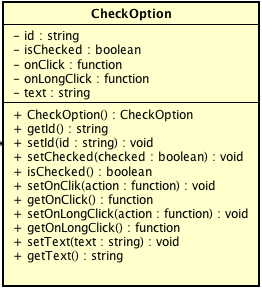
\includegraphics[scale=0.5]{Sezioni/SottosezioniST/img/CheckOption.png}
	\caption{monolith::component::widget::checklist::option::CheckOption}
\end{figure}

\begin{itemize}
\item \textbf{Descrizione}: La classe rappresenta lo stato, comprensivo di testo e id, di un ChecklistItemWidget.
\item \textbf{Utilizzo}: Viene utilizzata per ogni modifica di un ChecklistItemWidget o evento relativo ad esso.
\item \textbf{Attributi}:
	\begin{itemize}
	\item \textit{private id:string}\\
	Stringa identificativa della entry della checklist.
	\item \textit{private isChecked:boolean}\\
	Booleano che rappresenta lo stato del ChecklistItemWidget, ovvero se questo è spuntata o no.
	\item \textit{private text:string}\\
	Questa stringa rappresenta il testo associato al ChecklistItemWidget.
	\end{itemize}
\item \textbf{Metodi}:
	\begin{itemize}
	\item \textit{public CheckOption():CheckOption}\\
	Il costruttore della classe CheckOption.
	\item \textit{public getId():string}\\
	Ritorna l'id associato al ChecklistItemWidget.
	\item \textit{public setId(id:string):void}\\
	Imposta l'id della entry con il valore passato.
		\\ \textbf{Parametri}: \begin{itemize}
		\item \textit{id:string}\\
			Valore da impostare come id della entry.
		\end{itemize}
	\item \textit{public setChecked(checked:boolean):void}\\
	Spunta la entry o toglie la spunta da essa.
		\\ \textbf{Parametri}: \begin{itemize}
		\item \textit{checked:boolean}\\
		Il metodo spunta la entry se questo campo è true, toglie la spunta se è false.
		\end{itemize} 
	\item \textit{public isChecked():boolean}\\
	Ritorna true se la entry è spuntata, false altrimenti.
	\item \textit{public getText():string}\\
	Ritorna la stringa contentente il testo associato al ChecklistItemWidget.
	\item \textit{public setText(text:string):void}\\
	Imposta il testo associato alla entry della checklist.
		\\ \textbf{Parametri}: \begin{itemize}
		\item \textit{text:string}\\
		La stringa contentente il testo che verrà impostato come testo associato al ChecklistItemWidget.
		\end{itemize} 
	\item \textit{public changeStatus():boolean}\\
	Inverte lo stato del check (cioè se è spuntato toglie la spunta, e viceversa) e ritorna il booleano che rappresenta il nuovo stato.
	\end{itemize}
\end{itemize}

\subsubsection{monolith::component::widget::checklist::option::CheckStyle}

\label{monolith::component::widget::checklist::option::CheckStyle}
\begin{figure}[H]
	\centering
	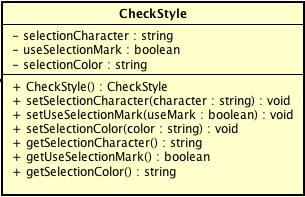
\includegraphics[scale=0.5]{Sezioni/SottosezioniST/img/CheckStyle.png}
	\caption{monolith::component::widget::checklist::option::CheckStyle}
\end{figure}

\begin{itemize}
\item \textbf{Descrizione}: La classe rappresenta lo stile con il quale vengono indicate le spunte su un ChecklistItemWidget.
\item \textbf{Utilizzo}: Il suo utilizzo è legato alla scelta visuale dello sviluppatore per quanto riguarda lo stile con il quale viene evidenziata una selezione nel ChecklistItemWidget.
\item \textbf{Attributi}:
	\begin{itemize}
	\item \textit{private selectionCharacter:string}\\
	Il carattere che viene utilizzato per la spunta del ChecklistItemWidget.
	\item \textit{private useSelectionMark:boolean}\\
	Se questo booleano è a true, le spunte verranno visualizzate con un carattere, altrimenti verranno visualizzate evidenziando il widget con un colore.
	\item \textit{private selectionColor:string}\\
	Rappresenta la stringa in esadecimale corrispondente al colore che è impostato per evidenziare i widget spuntati.
	\end{itemize}
\item \textbf{Metodi}:
	\begin{itemize}
	\item \textit{public CheckStyle():CheckStyle}\\
	Il costruttore della classe CheckStyle.
	\item \textit{public setSelectionCharacter(character:string):void}\\
	Imposta il carattere per la spunta delle entry della checklist.
		\\ \textbf{Parametri}: \begin{itemize}
		\item \textit{character:string}\\
		Il carattere scelto per visualizzare le spunte.
		\end{itemize} 
	\item \textit{public setUseSelectionMark(useMark:boolean):void}\\
	Imposta l'utilizzo del carattere o del colore per evidenziare la spunta di un ChecklistItemWidget.
		\\ \textbf{Parametri}: \begin{itemize}
		\item \textit{useMark:boolean)}\\
		Se questo booleano è a true, le spunte verranno visualizzate con un carattere, altrimenti verranno visualizzate evidenziando i widget con un colore.
		\end{itemize} 
	\item \textit{public setSelectionColor(color:string):void}\\
	Imposta il colore per evidenziare la spunta del widget.
		\\ \textbf{Parametri}: \begin{itemize}
		\item \textit{color:string}\\
		Rappresenta la stringa in esadecimale corrispondente al colore che verrà impostato per evidenziare la spunta del widget.
		\end{itemize} 
	\item \textit{public getSelectionCharacter():string}\\
	Ritorna il carattere che viene utilizzato per la spunta del widget.
	\item \textit{public getUseSelectionMark():boolean}\\
	Ritorna true se viene utilizzato il carattere per visualizzare la spunta, altrimenti false.
	\item \textit{public getSelectionColor():string}\\
	Ritorna la stringa in esadecimale corrispondente al colore che è impostato per evidenziare la spunta del widget.
	\end{itemize}
\end{itemize}

\subsubsection{monolith::component::widget::list::ListWidgetView}

\label{monolith::component::widget::list::ListWidgetView}
\begin{figure}[H]
	\centering
	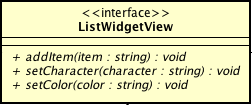
\includegraphics[scale=0.5]{Sezioni/SottosezioniST/img/ListWidgetView.png}
	\caption{monolith::component::widget::list::ListWidgetView}
\end{figure}

\begin{itemize}
\item \textbf{Descrizione}: Questa interfaccia rappresenta la view relativa ai widget di tipo lista.
\item \textbf{Utilizzo}: L'interfaccia viene utilizzata per disaccoppiare presenter e implementazione del widget, visualizza i dati che gli vengono passati dal presenter.
\item \textbf{Attributi}:
\item \textbf{Metodi}:
	\begin{itemize}
	\item \textit{public addItem(item:string):void}\\
	Aggiunge un oggetto alla lista.
		\\ \textbf{Parametri}: \begin{itemize}
		\item \textit{item:string}\\
		Il testo dell'oggetto da aggiungere alla lista.
		\end{itemize} 
	\item \textit{public setCharacterNumber():void}\\
	Cambia l'indicatore della lista impostando la visualizzazione con i numeri.
	\item \textit{public setCharacterCircle():void}\\
	Cambia l'indicatore della lista impostando la visualizzazione con i pallini.
	\item \textit{public setCharacterDash():void}\\
	Cambia l'indicatore della lista impostando la visualizzazione con i trattini.
	\item \textit{public setColor(color:string):void}\\
		Imposta il colore del carattere utilizzato per indicare un elemento nella lista.
		\\ \textbf{Parametri}: \begin{itemize}
		\item \textit{color:string}\\
		Codice esadecimale corrispondente al colore con il quale verrà colorato il carattere utilizzato per indicare un elemento nella lista.
		\end{itemize} 
	\item \textit{public getColor():string}\\
	Ritorna la stringa esadecimale corrispondente al colore con il quale verrà colorato il carattere utilizzato per indicare un elemento nella lista.
	\item \textit{public getOptions():List<string>}\\
	Ritorna un array contenente tutti gli elementi presenti all'interno della lista.
	\item \textit{public getCharacter():string}\\
	Ritorna il carattere utilizzato attualmente come indicatore per gli elementi della lista.
	\end{itemize}
\end{itemize}

\subsubsection{monolith::component::widget::list::view::ListWidget}

\label{monolith::component::widget::list::view::ListWidget}
\begin{figure}[H]
	\centering
	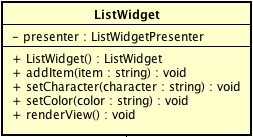
\includegraphics[scale=0.5]{Sezioni/SottosezioniST/img/ListWidget.png}
	\caption{monolith::component::widget::list::view::ListWidget}
\end{figure}

\begin{itemize}
\item \textbf{Descrizione}: Questa classe rappresenta un widget lista, un elenco di oggetti senza ordine, implementando l'interfaccia ListWidgetView.
\item \textbf{Utilizzo}: Implementando i metodi di ListWidgetView questa classe viene utilizzata al momento della creazione e della personalizzazione del widget lista e del suo contenuto.
\item \textbf{Attributi}:
	\begin{itemize}
	\item \textit{private presenter:ListWidgetPresenter}\\
	Il presenter associato al widget lista, al quale questa classe delega la gestione del comportamento del widget stesso.
	\end{itemize}
\item \textbf{Metodi}:
	\begin{itemize}
	\item \textit{public ListWidget():ListWidget}\\
	Il costruttore della class ListWidget.
	\item \textit{public addItem(item:string):void}\\
	Aggiunge un oggetto alla lista.
		\\ \textbf{Parametri}: \begin{itemize}
		\item \textit{item:string}\\
		Il testo dell'oggetto da aggiungere alla lista.
		\end{itemize} 
	\item \textit{public setCharacterNumber():void}\\
	Cambia l'indicatore della lista impostando la visualizzazione con i numeri.
	\item \textit{public setCharacterCircle():void}\\
	Cambia l'indicatore della lista impostando la visualizzazione con i pallini.
	\item \textit{public setCharacterDash():void}\\
	Cambia l'indicatore della lista impostando la visualizzazione con i trattini.
	\item \textit{public setColor(color:string):void}\\
		Imposta il colore del carattere utilizzato per indicare un elemento nella lista.
		\\ \textbf{Parametri}: \begin{itemize}
		\item \textit{color:string}\\
		Codice esadecimale corrispondente al colore con il quale verrà colorato il carattere utilizzato per indicare un elemento nella lista.
		\end{itemize} 
	\item \textit{public getColor():string}\\
	Ritorna la stringa esadecimale corrispondente al colore con il quale verrà colorato il carattere utilizzato per indicare un elemento nella lista.
	\item \textit{public getOptions():List<string>}\\
	Ritorna un array contenente tutti gli elementi presenti all'interno della lista.
	\item \textit{public getCharacter():string}\\
	Ritorna il carattere utilizzato attualmente come indicatore per gli elementi della lista.
	\item \textit{public renderView():HtmlDOMElement}\\
	Restituisce l'elemento DOM rappresentante il widget.
	\end{itemize}
\end{itemize}

\subsubsection{monolith::component::widget::list::presenter::ListWidgetPresenter}

\label{monolith::component::widget::list::presenter::ListWidgetPresenter}
\begin{figure}[H]
	\centering
	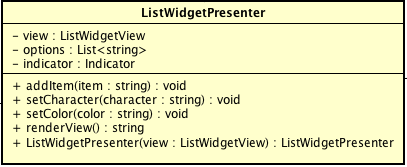
\includegraphics[scale=0.5]{Sezioni/SottosezioniST/img/ListWidgetPresenter.png}
	\caption{monolith::component::widget::list::presenter::ListWidgetPresenter}
\end{figure}

\begin{itemize}
\item \textbf{Descrizione}: Questa classe rappresenta il presenter per i widget di tipo lista.
\item \textbf{Utilizzo}: Il presenter fa da tramite tra l'implementazione del widget e la view, formattando i dati che verranno visualizzati nella view e manipolando gli input dell'utente per eseguire le operazioni predisposte.
\item \textbf{Attributi}:
	\begin{itemize}
	\item \textit{private view:ListWidgetView}\\
	La view associata al presenter.
	\item \textit{private options:List<string>}\\
	Questa collezione di stringhe rappresenta l'elenco di oggetti appartenenti alla lista.
	\item \textit{private indicator:Indicator}\\
	Il simbolo impostato per indicare gli oggetti della lista.
	\item \textit{private map:canMap}\\
	La mappa della libreria map necessaria alle funzioni del widget.
	\item \textit{private dom:HtmlDOMElement}\\
	L'elemento dom che contiene il widget lista in questione.
	\end{itemize}
\item \textbf{Metodi}:
	\begin{itemize}
	\item \textit{public ListWidgetPresenter(view:ListWidgetView):ListWidgetPresenter}\\
	Il costruttore della classe ListWidgetPresenter.
		\\ \textbf{Parametri}: \begin{itemize}
		\item \textit{view:ListWidgetView}\\
		La view necessaria alla costruzione del presenter.
		\end{itemize} 
	\item \textit{public addItem(item:string):void}\\
	Aggiunge un oggetto alla lista.
		\\ \textbf{Parametri}: \begin{itemize}
		\item \textit{item:string}\\
		Il testo dell'oggetto da aggiungere alla lista.
		\end{itemize} 
	\item \textit{public setCharacterNumber():void}\\
	Cambia l'indicatore della lista impostando la visualizzazione con i numeri.
	\item \textit{public setCharacterCircle():void}\\
	Cambia l'indicatore della lista impostando la visualizzazione con i pallini.
	\item \textit{public setCharacterDash():void}\\
	Cambia l'indicatore della lista impostando la visualizzazione con i trattini.
	\item \textit{public setColor(color:string):void}\\
		Imposta il colore del carattere utilizzato per indicare un elemento nella lista.
		\\ \textbf{Parametri}: \begin{itemize}
		\item \textit{color:string}\\
		Codice esadecimale corrispondente al colore con il quale verrà colorato il carattere utilizzato per indicare un elemento nella lista.
		\end{itemize} 
	\item \textit{public getColor():string}\\
	Ritorna la stringa esadecimale corrispondente al colore con il quale verrà colorato il carattere utilizzato per indicare un elemento nella lista.
	\item \textit{public getOptions():List<string>}\\
	Ritorna un array contenente tutti gli elementi presenti all'interno della lista.
	\item \textit{public getCharacter():string}\\
	Ritorna il carattere utilizzato attualmente come indicatore per gli elementi della lista.
	\item \textit{public renderView():HtmlDOMElement}\\
	Restituisce l'elemento DOM rappresentante il widget.
	\end{itemize}
\end{itemize}

\subsubsection{monolith::component::widget::list::option::Indicator}

\label{monolith::component::widget::list::option::Indicator}
\begin{figure}[H]
	\centering
	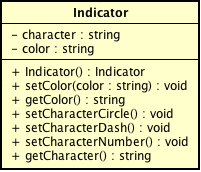
\includegraphics[scale=0.5]{Sezioni/SottosezioniST/img/Indicator.png}
	\caption{monolith::component::widget::list::option::Indicator}
\end{figure}

\begin{itemize}
\item \textbf{Descrizione}: Questa classe rappresenta l'indicatore per gli oggetti di un widget lista.
\item \textbf{Utilizzo}: Ogni lista ha un indicatore per i suoi oggetti, e questa classe fornisce gli strumenti per personalizzarlo.
\item \textbf{Attributi}:
	\begin{itemize}
	\item \textit{private character:string}\\
	Il simbolo impostato per indicare gli oggetti della lista.
	\item \textit{private color:string}\\
	Rappresenta la stringa in esadecimale corrispondente al colore che è impostato per gli indicatori.
	\end{itemize}
\item \textbf{Metodi}:
	\begin{itemize}
	\item \textit{public Indicator():Indicator}\\
	Il costruttore della classe Indicator.
	\item \textit{public setCharacterNumber():void}\\
	Cambia l'indicatore della lista impostando la visualizzazione con i numeri.
	\item \textit{public setCharacterCircle():void}\\
	Cambia l'indicatore della lista impostando la visualizzazione con i pallini.
	\item \textit{public setCharacterDash():void}\\
	Cambia l'indicatore della lista impostando la visualizzazione con i trattini.
	\item \textit{public setColor(color:string):void}\\
	Imposta il colore degli indicatori.
		\\ \textbf{Parametri}: \begin{itemize}
		\item \textit{color:string}\\
		la stringa in esadecimale corrispondente al colore che verrà impostato per gli indicatori.
		\end{itemize} 
	\item \textit{public getCharacter():string}\\
	Ritorna il simbolo usato per indicare gli oggetti della lista.
	\item \textit{public getColor():string}\\
	Ritorna la stringa in esadecimale corrispondente al colore che è impostato per gli indicatori.
	\end{itemize}
\end{itemize}

\subsubsection{monolith::component::widget::image::ImageWidgetView}

\label{monolith::component::widget::image::ImageWidgetView}
\begin{figure}[H]
	\centering
	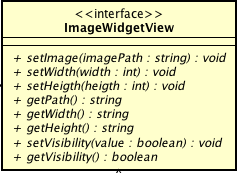
\includegraphics[scale=0.5]{Sezioni/SottosezioniST/img/ImageWidgetView.png}
	\caption{monolith::component::widget::image::ImageWidgetView}
\end{figure}

\begin{itemize}
\item \textbf{Descrizione}: Questa interfaccia rappresenta la view relativa ai widget di tipo immagine.
\item \textbf{Utilizzo}: L'interfaccia viene utilizzata per disaccoppiare presenter e implementazione del widget.
\item \textbf{Attributi}:
\item \textbf{Metodi}:
	\begin{itemize}
	\item \textit{public setImage(imagePath:string):void}\\
	Imposta il percorso nel file system che porta all'immagine che si vuole inserire nel widget.
		\\ \textbf{Parametri}: \begin{itemize}
		\item \textit{imagePath:string}\\
		Il percorso dell'immagine.
		\end{itemize} 
	\item \textit{public setHeight(height:int):void}\\
	Imposta l'altezza dell'immagine.
		\\ \textbf{Parametri}: \begin{itemize}
		\item \textit{height:int}\\
		L'altezza dell'immagine che si vuole impostare in pixel.
		\end{itemize} 
	\item \textit{public setWidth(width:int):void}\\
	Imposta la larghezza dell'immagine.
		\\ \textbf{Parametri}: \begin{itemize}
		\item \textit{width:int}\\
		La larghezza dell'immagine che si vuole impostare in pixel.
		\end{itemize} 
	\item \textit{public getPath():string}\\
	Ritorna la stringa contenente il percorso che porta all'immagine.
	\item \textit{public getHeigth():string}\\
	Ritorna l'altezza dell'immagine.
	\item \textit{public getWidth():string}\\
	Ritorna la larghezza dell'immagine.
	\end{itemize}
\end{itemize}

\subsubsection{monolith::component::widget::image::view::ImageWidget}

\label{monolith::component::widget::image::view::ImageWidget}
\begin{figure}[H]
	\centering
	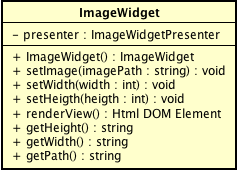
\includegraphics[scale=0.5]{Sezioni/SottosezioniST/img/ImageWidget.png}
	\caption{monolith::component::widget::image::view::ImageWidget}
\end{figure}

\begin{itemize}
\item \textbf{Descrizione}: Questa classe rappresenta un widget immagine, implementando l'interfaccia ImageWidgetView.
\item \textbf{Utilizzo}: Implementando i metodi di ImageWidgetView questa classe viene utilizzata al momento della creazione e della personalizzazione del widget immagine e del suo contenuto.
\item \textbf{Attributi}:
	\begin{itemize}
	\item \textit{private presenter:ImageWidgetPresenter}\\
	Il presenter associato al widget immagine, al quale questa classe delega la gestione del comportamento del widget stesso.
	\end{itemize}
\item \textbf{Metodi}:
	\begin{itemize}
	\item \textit{public ImageWidget():ImageWidget}\\
	Il costruttore della classe ImageWidget.
	\item \textit{public setImage(imagePath:string):void}\\
	Imposta il percorso nel file system che porta all'immagine che si vuole inserire nel widget.
		\\ \textbf{Parametri}: \begin{itemize}
		\item \textit{imagePath:string}\\
		Il percorso dell'immagine.
		\end{itemize} 
	\item \textit{public setHeight(height:int):void}\\
	Imposta l'altezza dell'immagine.
		\\ \textbf{Parametri}: \begin{itemize}
		\item \textit{height:int}\\
		L'altezza dell'immagine che si vuole impostare in pixel.
		\end{itemize} 
	\item \textit{public setWidth(width:int):void}\\
	Imposta la larghezza dell'immagine.
		\\ \textbf{Parametri}: \begin{itemize}
		\item \textit{width:int}\\
		La larghezza dell'immagine che si vuole impostare in pixel.
		\end{itemize} 
	\item \textit{public getPath():string}\\
	Ritorna la stringa contenente il percorso che porta all'immagine.
	\item \textit{public getHeigth():string}\\
	Ritorna l'altezza dell'immagine.
	\item \textit{public getWidth():string}\\
	Ritorna la larghezza dell'immagine.
	\item \textit{public renderView():HtmlDOMElement}\\
	Restituisce l'elemento DOM rappresentante il widget.
	\end{itemize}
\end{itemize}

\subsubsection{monolith::component::widget::image::presenter::ImageWidgetPresenter}

\label{monolith::component::widget::image::presenter::ImageWidgetPresenter}
\begin{figure}[H]
	\centering
	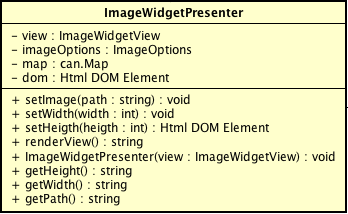
\includegraphics[scale=0.5]{Sezioni/SottosezioniST/img/ImageWidgetPresenter.png}
	\caption{monolith::component::widget::image::presenter::ImageWidgetPresenter}
\end{figure}

\begin{itemize}
\item \textbf{Descrizione}: Questa classe rappresenta il presenter per i widget di tipo lista.
\item \textbf{Utilizzo}: Il presenter fa da tramite tra l'implementazione del widget e la view, formattando i dati che verranno visualizzati nella view e manipolando gli input dell'utente per eseguire le operazioni predisposte.
\item \textbf{Attributi}:
	\begin{itemize}
	\item \textit{private view:ImageWidgetView}\\
	La view associata al presenter.
	\item \textit{private imageOptions:ImageOptions}\\
	Contiene le impostazioni attuali del widget.
	\item \textit{private map:canMap}\\
	La mappa della libreria map necessaria alle funzioni del widget.
	\item \textit{private dom:HtmlDOMElement}\\
	Il dom che rappresenta il widget.
	\end{itemize}
\item \textbf{Metodi}:
	\begin{itemize}
	\item \textit{public ImageWidgetPresenter(view:ImageWidgetView):ImageWidgetPresenter}\\
	Il costruttore della classe ImageWidgetPresenter.
		\\ \textbf{Parametri}: \begin{itemize}
		\item \textit{view:ImageWidgetView}\\
		La view necessaria alla costruzione del presenter.
		\end{itemize}
	\item \textit{public setImage(imagePath:string):void}\\
	Imposta il percorso nel file system che porta all'immagine che si vuole inserire nel widget.
		\\ \textbf{Parametri}: \begin{itemize}
		\item \textit{imagePath:string}\\
		Il percorso dell'immagine.
		\end{itemize} 
	\item \textit{public setHeight(height:int):void}\\
	Imposta l'altezza dell'immagine.
		\\ \textbf{Parametri}: \begin{itemize}
		\item \textit{height:int}\\
		L'altezza dell'immagine che si vuole impostare in pixel.
		\end{itemize} 
	\item \textit{public setWidth(width:int):void}\\
	Imposta la larghezza dell'immagine.
		\\ \textbf{Parametri}: \begin{itemize}
		\item \textit{width:int}\\
		La larghezza dell'immagine che si vuole impostare in pixel.
		\end{itemize} 
	\item \textit{public getPath():string}\\
	Ritorna la stringa contenente il percorso che porta all'immagine.
	\item \textit{public getHeigth():string}\\
	Ritorna l'altezza dell'immagine.
	\item \textit{public getWidth():string}\\
	Ritorna la larghezza dell'immagine.
	\item \textit{public renderView():HtmlDOMElement}\\
	Restituisce l'elemento DOM rappresentante il widget.
	\end{itemize}
\end{itemize}

\subsubsection{monolith::component::widget::image::option::ImageOptions}

\label{monolith::component::widget::image::option::ImageOptions}
\begin{figure}[H]
	\centering
	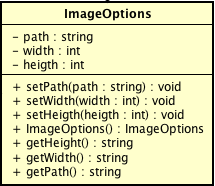
\includegraphics[scale=0.5]{Sezioni/SottosezioniST/img/ImageOptions.png}
	\caption{monolith::component::widget::image::option::ImageOptions}
\end{figure}

\begin{itemize}
\item \textbf{Descrizione}: Questa classe rappresenta le impostazioni di un widget immagine.
\item \textbf{Utilizzo}: Ogni cambiamento delle impostazioni di visualizzazione di un widget immagine coinvolge questa classe.
\item \textbf{Attributi}:
	\begin{itemize}
	\item \textit{private path:string}\\
	Il percorso dell'immagine.
	\item \textit{private width:int}\\
	L'altezza dell'immagine. 
	\item \textit{private height:int}\\
	La larghezza dell'immagine. 
	\end{itemize}
\item \textbf{Metodi}:
	\begin{itemize}
	\item \textit{public ImageOptions():ImageOptions}\\
	Il costruttore della classe ImageOptions.
	\item \textit{public setPath(path:string):void}\\
	Imposta il percorso nel file system che porta all'immagine che si vuole inserire nel widget.
		\\ \textbf{Parametri}: \begin{itemize}
		\item \textit{path:string}\\
		Il percorso dell'immagine.
		\end{itemize} 
	\item \textit{public setHeight(height:int):void}\\
	Imposta l'altezza dell'immagine.
		\\ \textbf{Parametri}: \begin{itemize}
		\item \textit{height:int}\\
		L'altezza dell'immagine che si vuole impostare  in pixel.
		\end{itemize} 
	\item \textit{public setWidth(width:int):void}\\
	Imposta la larghezza dell'immagine.
		\\ \textbf{Parametri}: \begin{itemize}
		\item \textit{width:int}\\
		La larghezza dell'immagine che si vuole impostare  in pixel.
		\end{itemize} 
	\item \textit{public getPath():string}\\
	Ritorna la stringa contenente il percorso che porta all'immagine.
	\item \textit{public getHeigth():string}\\
	Ritorna l'altezza dell'immagine.
	\item \textit{public getWidth():string}\\
	Ritorna la larghezza dell'immagine.
	\end{itemize}
\end{itemize}